
\title{Hierarchical Controller Architecture in Software Defined Networks}
\author{
        Author 1 \\
            \and
        Author 2\\
        %UIUC\\
			\and
		Author 3\\
}
\date{\today}

\documentclass[10pt, twocolumn]{article}
\usepackage{url,graphicx,tabularx,array,geometry, caption, subcaption, float}
%-- Commands for header
\renewcommand{\title}[1]{\textbf{#1}\\}
\renewcommand{\line}{\begin{tabularx}{\textwidth}{X>{\raggedleft}X}\hline\\\end{tabularx}\\[-0.10cm]}
\newcommand{\leftright}[2]{\begin{tabularx}{\textwidth}{X>{\raggedleft}X}#1%
& #2\\\end{tabularx}\\[-0.10cm]}

\newcolumntype{L}[1]{>{\raggedright\let\newline\\\arraybackslash\hspace{0pt}}m{#1}}
\newcolumntype{C}[1]{>{\centering\let\newline\\\arraybackslash\hspace{0pt}}m{#1}}
\newcolumntype{R}[1]{>{\raggedleft\let\newline\\\arraybackslash\hspace{0pt}}m{#1}}


\begin{document}
\maketitle
\begin{abstract}
Network control plane, in Software Defined Networks (SDN), provides a global view of the physical network to control applications. Regardless of this abstraction, the control plane itself must inevitably be a distributed system, with multiple nodes called controllers, to achieve desired level of scalability, reliability and responsiveness. 

Conventional control plane architecture involves multiple peer controllers, each operating on a subset of network and maintaining a global view of the entire network. We propose a different architecture where controllers are arranged in a hierarchy and only view a part of the network. Limiting the view of controllers significantly reduces communication overhead while modestly compromising on optimality. We simulated both architectures on historical Hadoop traces from Facebook and observed that hierarchical architecture reduces communication overhead by an order of magnitude (90.5\%) while deviating from optimal results by 17.4\% for routing application and 12.8\% for Traffic Engineering (TE) application. 

Besides, we also propose an optimization in conventional flat controller architecture and shows preliminary results on a dummy topology. 
\end{abstract}

\section{Introduction}
%Forwarding or data plane consists of a collection of forwarding elements (switches), connected to form a network, which is inherently distributed in nature. Control plane consists of a collection of control elements, which install forwarding rules on forwarding elements as dictated by control logic or application, running on control elements. Some classes of control applications are routing, traffic engineering (TE), enforcing network policies, etc. 
In traditional networks, there is a tight coupling and a one-to-one mapping between control elements and forwarding elements, with one pair on each switch. Besides, the role of control elements had been trivial, which is to merely install instructions given by control application on corresponding forwarding element as forwarding rules. It is the control application which runs distributed protocols to synchronize the state of forwarding elements. The design of these distributed protocols differs from application to application. For example, link state routing makes switches share their neighbors while distance vector routing makes switches share their routing tables.

The emergence of Software Defined Networks (SDN) has induced a separation between forwarding and control elements and has significantly improved the role of the control plane. The control elements may no longer be present on the switches but move to a separate device called a controller, and use predefined protocol such as OpenFlow \cite{openflow}, to install forwarding rules. There may be a one-to-many mapping from controllers to switches. At one extreme, control plane may provide a control application with the global network view, which can then be implemented as a centralized application, rather than a distributed one. Regardless of this abstraction, the control plane itself must inevitably be a distributed system, with multiple controllers, to achieve desired level of scalability, reliability and responsiveness.

Conventional control plane architectures involve multiple peer controllers, where each controller operates on a subset of switches and maintains a global view of the entire network, which is exposed to the control application. We refer to such an architecture as \emph{flat controller architecture}. Underlying network state is shared with other controllers through distributed state dissemination frameworks such as distributed transactional databases or Distributed Hash Tables (DHT). Consequently, such an architecture results in huge communication overhead between controllers, which may hinders the scalability of the system. Besides, network state inconsistency is quite common in flat architecture which degrades the application performance significantly \cite{logically-centralized}.

The state inconsistency and huge communication overhead problem arises from the fact that each controller tries to maintain the complete global view of the network. Motivated by this observation, we propose a hierarchical controller architecture, in which controllers are arranged in a tree structure and exposes a switch abstraction to its parent. We show that hierarchical architecture significantly reduces the communication overhead between controllers while modestly compromising on optimality.     

\paragraph{Outline}
The remainder of this article is organized as follows. Section~\ref{sec:hierarchical} presents Hierarchical Controller Architecture. We discuss implementation details and present experimental results in section~\ref{sec:eval}. In section~\ref{sec:timestamps}, we present an optimization to conventional flat controller architecture. We discuss pros and cons of proposed architecture in section \ref{sec:discuss}. Related work is discussed in section~\ref{sec:related}. We conclude the paper in section \ref{sec:conc}, followed by future work in section \ref{sec:future}.  

\section{Hierarchical Controller Architecture}
\label{sec:hierarchical}
We propose a new control plane architecture in which controllers are arranged in the form of a tree over the physical network. We will start by describing an important building block of the architecture, called switch abstraction.

\subsection{One switch abstraction}
\label{subsec:aggr}
A controller aggregates its underlying network and behaves as one logical switch, with huge number of ports. This logical switch supports control plane protocols such as OpenFlow\cite{openflow,of-spec}, and can be controlled by an external entity (referred to as parent controller) to install forwarding rules. One switch abstraction has two parts, (i) compressing the underlying network state to represent a single switch, and (ii) translating instructions (forwarding rules) from the abstract switch to the underlying network. We present these separately below.
\subsubsection{Compression}
The primary switch abstraction comes by compressing the network into one node. Given an underlying network for a controller, the abstract switch exposed by it contains all the ports which are connected to switches outside the network. Such ports are referred to as \emph{external} ports. Conversely, ports which are connected to ports in the same network are not exposed (hidden away from abstraction) and are referred to as \emph{internal} ports. \emph{External} ports form the \emph{ingress} and \emph{egress} ports for the abstract switch. The switch abstraction maintains a list of these abstract ports, which can be (uniquely) mapped to the ports of the underlying network. This basic abstraction is sufficient for a simple control application, but we require more features for a rich and complete experience. A few such abstractions are presented below.
\begin{enumerate}
    \item \emph{Host compression}:
    Hosts in the underlying network are considered as external entities, which are exposed as hosts connected to the abstract switch. Ports which connect to hosts are considered to be \emph{external} ports. However, if the number of hosts in the underlying network is too large, exposing a list of all hosts could result in inefficient compression. Host compression can be performed in two ways, depending on the host IP distribution and the network being considered.
    \begin{itemize}
        \item \emph{IP compression} -
        Similar to the forwarding rules in an Internet router, if the IP addresses of the hosts are properly prefixed, a controller can compress host IPs and only provide prefixes to its parent controller. This works well only if the assignment of switches to controllers is uniform and in accordance with prefixes.
        \item \emph{Abstract host list} -
        A controller can expose an abstract host or list of hosts to its parent controller. The parent controller places rules for the abstract hosts in the peer controllers. This approach would be similar to LAN, and requires address translation while entering or leaving the underlying network. This is more flexible, but complicated, and can be used only when IP prefix compression fails.
    \end{itemize}
    \item \emph{Abstract flow table}:
        The basic flow table in a controller comprises of the rules placed by the parent controller. However, for a full OpenFlow functionality, we need to support counters and queries, as in OpenFlow switches. These responses, again, must be an aggregation of the network. To this end, we must be able to efficiently represent the flows from the underlying network and obtain statistics which can be exposed to the parent. We propose a data structure to maintain, aggregate and update view of the flows in section~\ref{subsubsec:aggr-data}.
\end{enumerate}

\subsubsection{Translation}
The major task of a controller is to translate messages from its parent controller to forwarding rules that can be implemented on switches in the underlying network. To this end, we extend the API for the control application to take in these rules as an additional input (Note: there is no standard northbound API between a controller and a control application as of today and each controller exposes its own unique API). The controller uses the underlying network state and its abstract flow table to decide the rules for its children. It forwards the packet to its parent if and only if it is unable to handle the packet with its given knowledge. Typically, for a new flow,
\begin{enumerate}
    \item If the destination is within the underlying network, or if the abstract flow table has rules to handle the destination, the controller places rules on the underlying network to create a flow from the origin (local host or an \emph{ingress} port) of the flow to the destination (local host or an \emph{egress} port) based on its policies.
    \item If the destination is unknown, it forwards the packet to its parent, but also holds onto a copy. Once the parent takes a decision and passes it as an OpenFlow rule, the controller translates it to the underlying network.
\end{enumerate}

\cite{one-big-switch} proposes algorithms to combine and translate end-to-end policies and routing policies to optimally place rules in switches. These algorithms can be used by control applications to optimally place rules, combining the abstract flow table and its local routing policies.

\subsubsection{Data structures}
\label{subsubsec:aggr-data}
In this section, we present data structures, maintained by a controller to translate instructions from parent controller to child switches and to translate network updates and messages from child switches to parent controller efficiently. Note that this is just one of the ways in which \emph{translation} can be enforced, which we have used in our implementation. We represent the underlying network as a graph $G$ with dummy external nodes connected to each of the exposed ports. For each external node $e$, we create and maintain a directed flow graph $F_e$ rooted at $e$ as an overlay graph on $G$. $e$ here represents the \emph{ingress} port. End hosts and other external nodes act as sinks for these flows. The external nodes represent the \emph{egress} ports.
For each pair of external nodes $e_{in}$ and $e_{out}$, we can create an aggregated flow table entry based on the flow graph $F_{e_{in}}$ for $e_{in}$. We propose this method to account for possible modifications in the packet headers along the paths (multiple paths are common based on routing policies) from the \emph{ingress} port to the \emph{egress} port which could prevent us from identifying same flows by just observing flows at the \emph{ingress} and \emph{egress} ports.
Other data structures which would aid to simplify updates and aggregation are
\begin{enumerate}
    \item \emph{Path Information} - A list of $n$ best paths for some definition of best. We consider paths with least hops, but this can be varied depending on the routing policies. This can be used to choose the best path to route from between an \emph{ingress} and \emph{egress} port based on routing policies.
    \item \emph{Link Information} - A list of pointers to the paths this link belongs to, and a list of flows that pass through this link. This can be used to obtain link utilizations to select routes with minimum maximum link utilization.
\end{enumerate}
One main difference between an abstract switch and an actual switch is the inequality of costs between two exposed ports. If parameters like hop counts are being considered, the internal routing costs must also be considered. This can be achieved by adding extra \emph{attributes} to pairs of external ports which can signify the internal costs which could be considered by the parent controller. This extra feature helps reduce the sub-optimality of this solution. However, it comes at the expense of needing to update costs of each pair of nodes on network changes.

\subsubsection{Modifications}
One major concern of routing is network modifications, mainly link failures. If the network is well connected, then an internal link failure can be handled by the local controller without affecting the parent controller. A parent controller only needs to concern if an exposed link is broken or if an underlying network is significantly broken, for example, if it was partitioned or the paths become extremely crowded. With the assumption that an underlying network capacity is greater than its exposed links, i.e. the internal network can handle full utilization of the exposed links, these concerns will be limited.

\subsection{Hierarchical arrangement}
We propose a new control plane architecture in which controllers are arranged in the form of a tree over the physical network as shown in figure ~\ref{fig:hierarchy}. Switches form the leaf nodes in the tree, while controllers form the internal nodes. An internal node acts as a switch for its parent and as a controller for its children. A controller's view does not span the whole network but only the network of its children. A node translates instructions (forwarding rules) from its parent controller to the forwarding rules for its underlying network. Similarly, network updates from the underlying network are translated into network updates arising from one switch abstraction of the given controller and are passed on to parent controller.

The abstraction described above represents a controller at any level of the hierarchy. The only difference between a root controller and an internal controller is the absence of incoming OpenFlow messages in the former, while the latter receives them from its parent. This simplifies the control application which can be agnostic to the hierarchical level it belongs to, as long as it can support incoming OpenFlow messages.

\begin{figure}
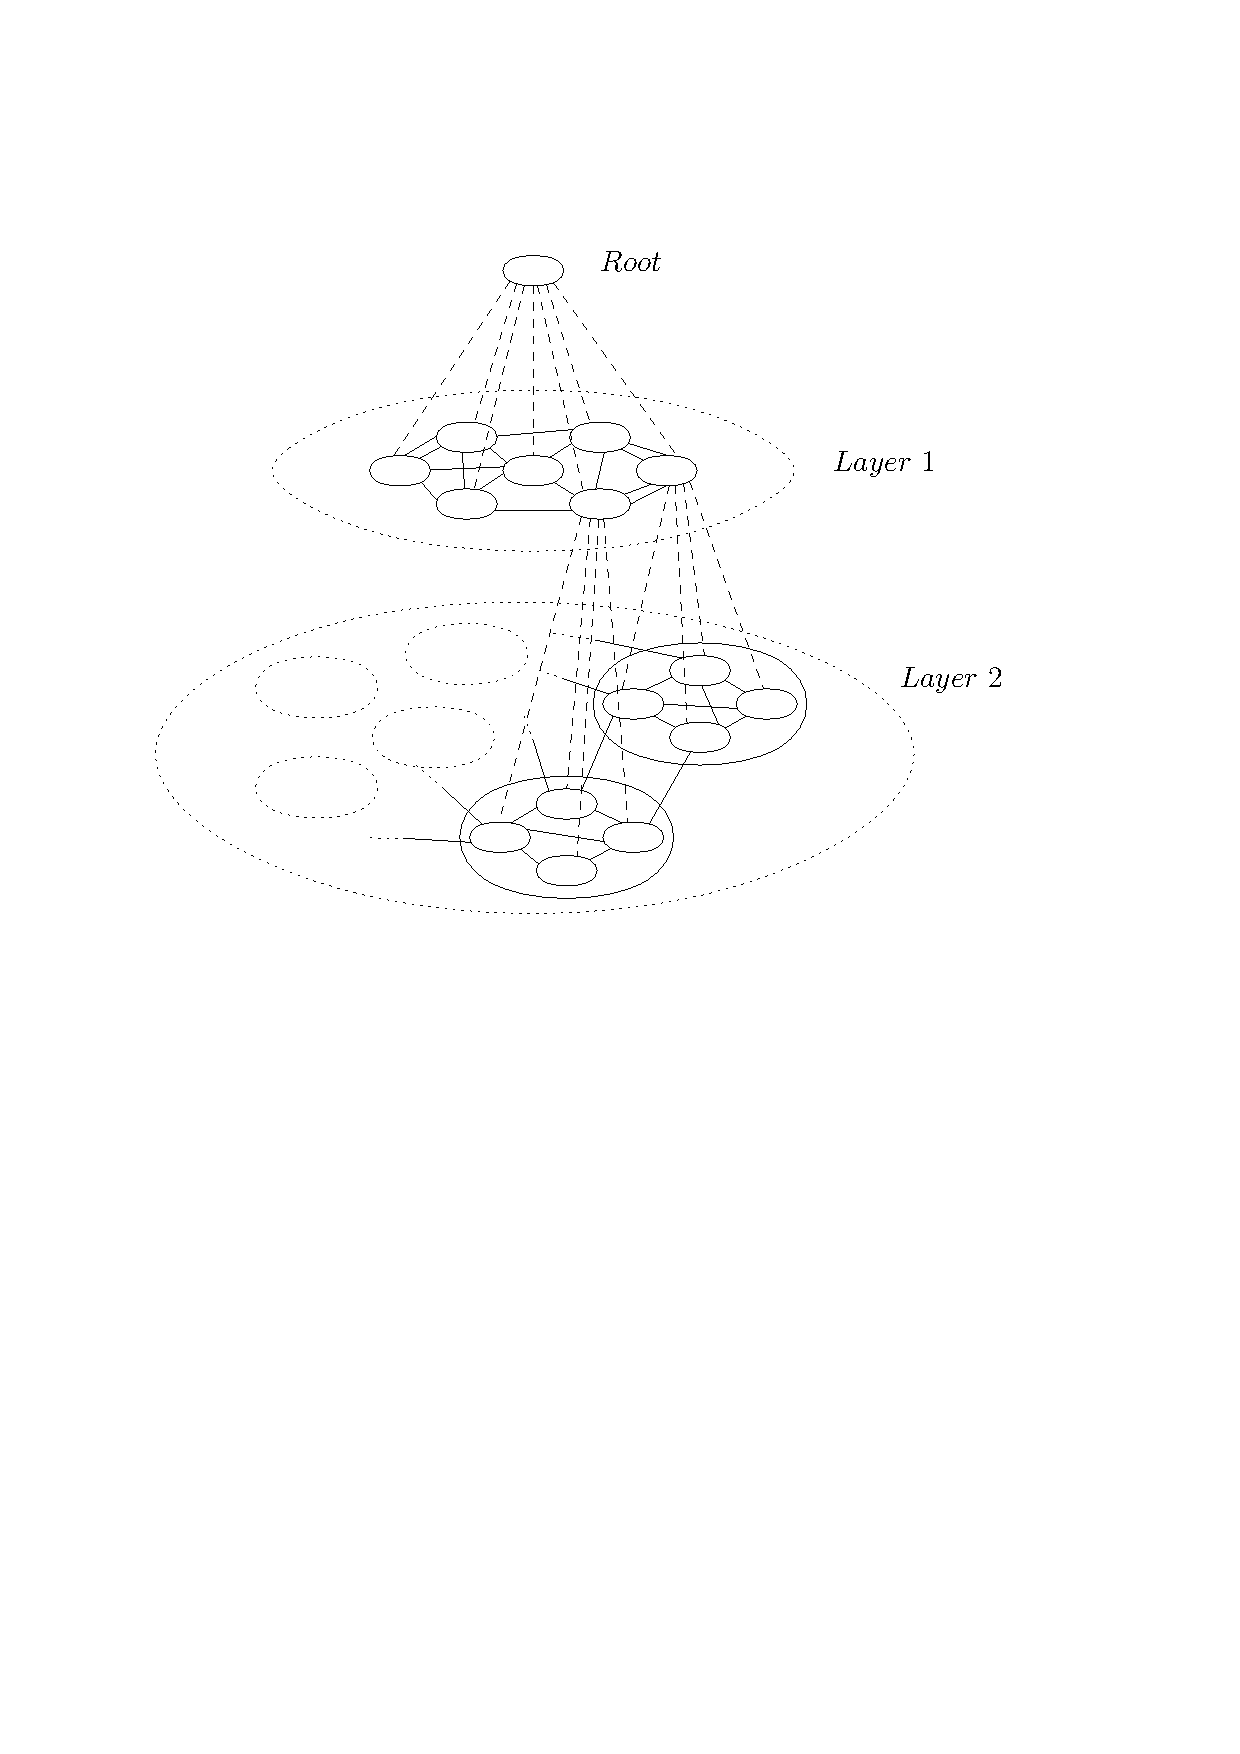
\includegraphics[scale=0.5]{hierarchy}
\caption{A 2-layer Hierarchical arrangement of controllers: Root controller manages the layer of controllers, which in-turn manages a subset of switches.}
\label{fig:hierarchy}
\end{figure}

\subsection{An example}
\label{example}
Let's consider an example to understand the benefits of hierarchical architecture. Let there be a TE control application running on $d$ controllers, with each controller operating on $d$ switches. Network state consists of current utilizations of all links. Whenever a new flow arrives, application choses a path with minimum maximum utilization and assigns it to the flow. Each time a path of length $l$ is assigned to the flow, there could be a maximum of $l*d$ link utilization updates and $l$ forwarding rule messages to be sent between controllers. Now, consider an architecture where controllers are arranged in hierarchical manner. There are $d+1$ controllers. The first $d$ controllers (called type 0) maintain $d$ switches each and acts as a switch to the last controller (called type 1), which in turn maintains the other $d$ controllers. Type 0 controllers keep track of link utilizations only for the links that connect it's children switches. Type 1 controller keep track of links that runs from switches belonging to one controller domain to another. Same TE control application runs on each controller. When a new flow arrives, a switch sends $packet\_in$ message to its type 0 controller. Type 0 controller checks if the path of the flow belongs entirely to its underlying network or not. If yes, it uses TE application to assign the path to the flow and no updates are sent to any controller. However, if the destination is outside its domain, type 0 controller sends a $packet\_in$ message to its parent controller. Parent controller uses TE control application to assign a paths of type 0 controllers. Forwarding rules are sent to type 0 controllers, which in turn sets up forwarding rules in their network. If the path length is $l$, there will be a maximum of $l+1$ forwarding rule messages between controllers and no link utilization updates. However, the path assigned might not be the one with minimum maximum utilization. This significant reduction in communication overhead comes at the cost of sub-optimality in the application performance. We show experimentally that the proposed architecture significantly reduces communication overhead while only modestly degrading application performance in the next section.

\section{Evaluation}
\label{sec:eval}
We simulated a dummy control application on both hierarchical and flat controller architectures, with same network topology and flow arrival distribution. The details of simulation, metrics and results are presented in this section.

\subsection{Implementation}
\label{sec:implementation}
We wrote our own simulator, which is available at \cite{simulator}. We did not use an existing simulator/controller such as Mininet\cite{mininet} with Floodlight\cite{floodlight} for the following two reasons: (1) Existing controllers lack the support for flexible controller architecture and are not suitable for hierarchical arrangement of controllers. Modifying existing controllers such as Floodlight to add support for one-switch abstraction (section~\ref{subsec:aggr}), is not a good idea because it requires code/design changes in their primitive modules. Besides, we were not looking for a feature rich controller at that point of time. (2) Existing simulators do not provide controls to regulate replication between controllers or to measure communication overhead (number of messages exchanged ) between controllers, which we needed for evaluation of control plane architecture. Given the above requirements, writing a simulator which provides one-switch abstraction support for the controllers was the best option.

There are three prime interfaces:
\begin{enumerate}
    \item {\it Switch Data Plane:} It is implemented by a switch to create forwarding elements to handle packet forwarding according to forwarding rules.
    \item {\it Switch Control Plane:} It is implemented by both controllers and switches and is used to establish connections with parent controllers to send packets which do not match any forwarding rule, to receive forwarding rules and send/receive other OpenFlow-like messages from parent controller.
    \item {\it Controller Control Plane:} It is implemented by controllers to establish connections to child switches/controllers. It is used to receive packets which do not match any forwarding rule and to send forwarding rules to child switches/controllers.
\end{enumerate}
Simulator defines two networks:
\begin{enumerate}
    \item {\it Data Network:} This network consists of all switches (and no controllers) connected through links.
    \item {\it Management Network:} This network consists of all controllers and switches connected through Controller - Switch Control Plane interfaces. This network allows flexible controller architecture, which could be hierarchical or flat.
\end{enumerate}

To observe the effect of different architectures in real world applications, we used SWIM project \cite{swim}, which provides synthetic representative test workloads  by sampling historical MapReduce cluster traces. The original trace comes from historical Hadoop traces on a 600 machine cluster at Facebook and spans $6$ months, and contains roughly $1$ million jobs. The representative trace file contains $\approx 6000$ jobs. The trace was simulated with a cluster of $600$ machines (as in the original cluster) connected through a network of $200$ switches and $10$ Gbps links. The cluster is divided into $10$ control domains, with $60$ hosts, $20$ switches and one controller for each domain. Each switch in a domain is connected to $1$ to $4$ switches within the same domain, with degree being chosen randomly. Each domain contains $2$ top-of-the-rack switches which inter-connect domains. For hierarchical architecture, there are $11$ controllers: $1$ controller per domain and $1$ root controller which manages the other $10$ controllers. While flat architecture consists of $10$ peer controllers, one for each domain.

Control application is a TE-cum-routing application. When a new flow arrives, control application finds the path with minimum maximum utilization and sets up forwarding rules (based on IP destination and incoming ports) along the path. If multiple such paths exist (which is frequently the case, due to a large network), shortest path (in term of number of hops) is chosen. This application runs on each controller in both hierarchical and flat architecture. However, in the hierarchical architecture, the view of application is limited and may consist of controllers or switches as forwarding elements, while in the flat architecture, control application is presented with global view of the network. For simplicity, we have kept network topology as static i.e. links/nodes do not fail and/or are not created during the simulation. For each Hadoop job, a dummy MapReduce application choses a directory, map and reduce nodes randomly in the network, thus, creating a number of flows which are handled by the control application running on controllers. The duration of flows depends on the bytes needed to transfer and the assigned rates.            

\subsection{Results}
\label{subsec:results}
We simulated the trace file for both flat and hierarchical architectures, with the same network topology and the same assignment of task nodes for each job. We calculated two metrics:
\begin{enumerate}
    \item The performance of control application which is measured as the length of the path (number of hops) assigned to flows (Figure ~\ref{fig:path}) and maximum link utilization encountered by the flow (Figure ~\ref{fig:util}). While the flat architecture gives optimal results, hierarchical architecture provides sub-optimal results. However, note that simulation provides instantaneous replication and thus eliminates network inconsistency between controller, which would  have otherwise, degraded the performance of flat architecture.
    \item Communication overhead during flow set up, which is measured in term of number of messages passed between switches and controllers as well as within controllers (Figure ~\ref{fig:msg}). The simulation assumes instant replication of network state between controllers.
\end{enumerate}
Results show that hierarchical architecture reduces the communication overhead between controllers by an order of magnitude while modestly deviating from optimal solution.

\begin{figure}[h]
\centering
\begin{subfigure}{.5\textwidth}
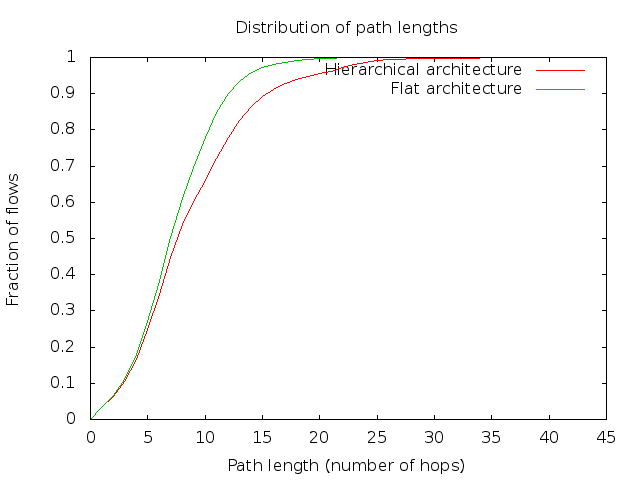
\includegraphics[scale=0.3]{path}
\caption{Application performance: path length for flows}
\label{fig:path}
\end{subfigure}

\begin{subfigure}{.5\textwidth}
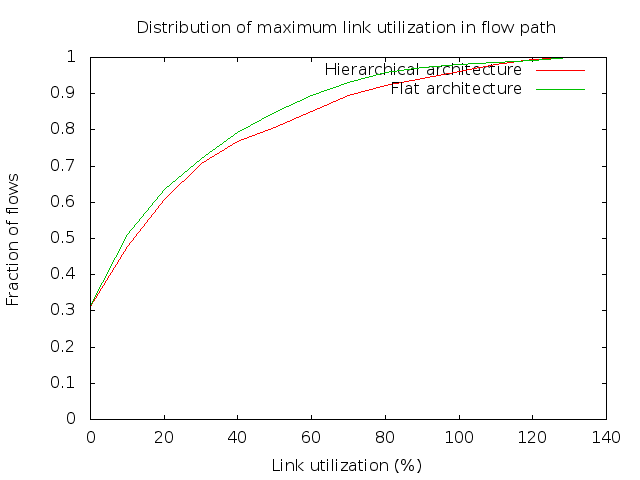
\includegraphics[scale=0.3]{util}
\caption{Application performance: Maximum link utilization for flows}
\label{fig:util}
\end{subfigure}
\caption{Application performance}
\end{figure}

\begin{figure}[h]
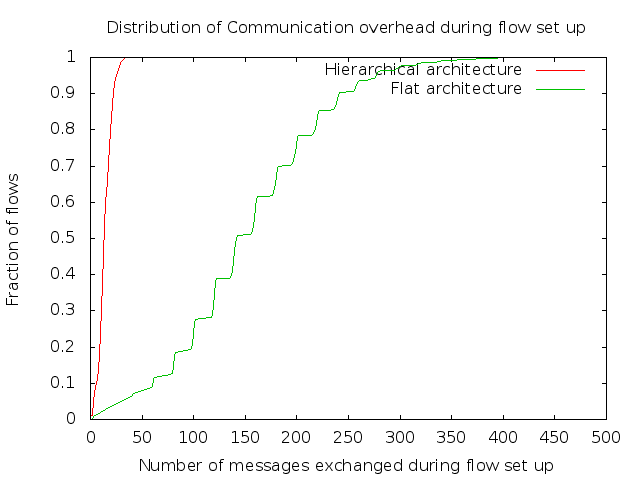
\includegraphics[scale=0.3]{msg}
\caption{Communication overhead per flow}
\label{fig:msg}
\end{figure}


\begin{table*}
\centering
\begin{tabular}{| L{4cm} | L{2cm} | L{3cm} | L{4cm} |}
\hline
& {Average path length} & {Average maximum utilization} & {Average communication overhead per flow} \\ \hline
Flat architecture & 7.81 & 24.62 & 153.54 \\ \hline
Hierarchical architecture & 9.17 & 27.78 & 14.52 \\ \hline
\end{tabular}
\caption{Comparison between performance of Flat and Hierarchical architecture.}
\end{table*}%



\section{Timestamps: An optimization for flat controller architecture}
\label{sec:timestamps}
In this section, we propose an optimization for flat controller architecture. 

\subsection{System model}
There are multiple peer controllers, managing different parts of the network and keeping a global view of the entire network. Network states are replicated between controllers, with some replication lag i.e. at a given instant of time network state of two controllers may be different or inconsistent. Network state could include a range of characteristics of underlying network including, topology, link utilizations, routing tables on switches, etc. However, for the purpose of this section, we will assume that network state only consists of link utilizations. Network state on a given controller consists of latest data for links that belong to it's domain, while it may contain stale data for other links. The topology is assumed to be static and is assumed to be known by all controllers. Source routing is used to route packets/flows to destination: when a new flow arrives at the ingress switch, it is sent to the parent controller, which calculates the route using control application and network state (at that point of time). This route is marked on the packet/flow.
  
\subsection{Optimization}
Let's say there are \emph{n} controller domains. Each controller domain, $i$ maintains a vector timestamp $T_{i}[1...n]$, where $T_{i}[j]$ contains the latest revision number of domain $j$'s network state (link utilizations), seen by domain $i$. Whenever links utilization is revised for links in domain $i$, the controller increments its own revision number $T_{i}[i]$ in the timestamp. Timestamps are sent along with the network state to other controllers for replication. During replication, a controller revises its timestamp with the incoming timestamp by taking maximum for each entry between the two timestamps. This is a general technique for any replicated system. Each router is updated with the latest timestamp of its parent controller. 

When a route is being set up, the controller prints its timestamp on packet header along with the route. When a router in a domain $i$ receives a flow with timestamp $T_{j}$ , it checks for any index $k$ such that $T_{j} [k] < T_{i} [k]$. For all such indices, it recalculates the part of the route which belongs to domain $k$ using its own network state. This is because these parts of the existing path were calculated on a stale network state.
  
\subsection{Evaluation}
We used a dummy topology to show the benefits of timestamps. There are three controller domains 1, 2 and 3, with domain 2 connecting the other two domains. Flows arrive randomly between domain 1 and domain 3 and are routed through domain 2. Link Balancer Controller \cite{logically-centralized} runs on each controller as a control application: when a new flow arrives, a path which minimizes the maximum link utilization is assigned to the flow.

\begin{figure}

\begin{subfigure}{.5\textwidth}
 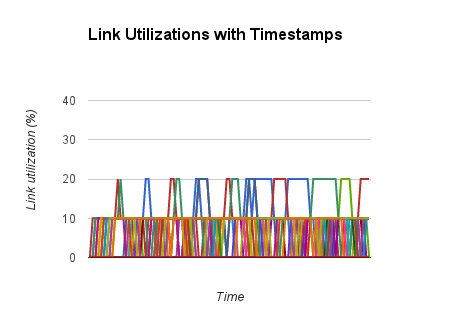
\includegraphics[scale=0.4]{chart_1}
\end{subfigure}
\begin{subfigure}{.5\textwidth}
 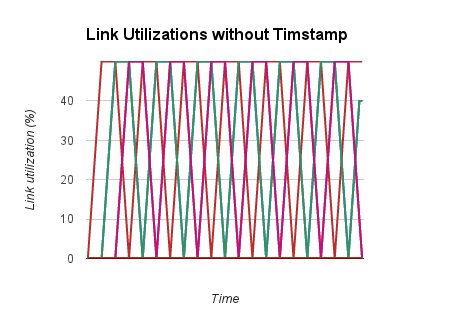
\includegraphics[scale=0.4]{chart_2}
\end{subfigure}
\caption{Comparison of Link utilizations with/without Timestamp optimization}
\label{fig:timestamp}
\end{figure}

Results (Figure \ref{fig:timestamp}) shows that using timestamp could improve control application's performance. However, these are only preliminary results on a dummy topology and does not give any indication of the magnitude of improvement. Going ahead, we plan to evaluate timestamp optimization on a bigger topology with real world flow arrival data. 

\section{Discussion}
\label{sec:discuss}
Hierarchical architecture provides several benefits.
\begin{enumerate}
    \item Compared to a flat distributed controller architecture, this architecture will have faster flow setup times, in general. In a flat architecture, flow setup requires one round trip between switch and controller for each of the controller domains (say $n$) the packet travels through. However, in a hierarchical architecture, the packet is forwarded up to a level where the entire path is under one controller and then the rules are installed in all the controllers. On average, this is $O(log\;n)$ levels up and thus takes significantly less time to setup. Worst case, however, could be when the two nodes are close to each other physically but belong to different controllers up till the root.
    \item Link modifications are in general handled locally by the immediate controller and other controllers are not affected by it. So, there are in general no messages or state inconsistencies, as these networks do not have a global state to create inconsistencies!
    \item As long as a control application follows the protocol, the internal routing mechanisms do not create any inconsistencies. In flat architecture where each controller takes a global decision but acts on a local scope, each controller must behave and take decisions exactly the same way. Thus, with our architecture, different controllers can run different control applications, without affecting the network. This has several benefits in itself.
        \begin{enumerate}
            \item A control application can be updated independent of the remaining network and not cause global disruptions. There might, however, be flow setup delays which are to be expected.
            \item Different routing strategies and network policies can be implemented in different segments of the network. For example, one controller could route using MPLS, while another uses destination addresses.
            \item Networks with different managements can be brought together using this architecture. Each network can follow its own network policies and selectively expose its \emph{ingress} and \emph{egress} ports to the parent controller.
        \end{enumerate}
    \item The view is simplified and thus decisions can be taken quickly, only for a small number of nodes at each level.
\end{enumerate}

This architecture, however, in not a panacea for scalable distributed controller architectures as simplifying the network comes at the cost of losing optimality. We still believe that the reduction is performance is modest compared to the advantages it offers.

\section{Related Work}
\label{sec:related}
Owing to the performance, reliability and scalability issues faced by single controller architectures, distributed controller architectures have been studied and implemented in various flavors. Most of them aim for a logically centralized global view of the network, while other provide a distributed framework and leave design choices to the control application. Some of them are discussed in this discussion.

Hyperflow\cite{hyperflow} has a logically centralized but physically distributed controller architecture. It localizes decision making in individual controllers by passively synchronizing the global network view. The control application is agnostic to the underlying architecture and takes a global decision, though the effect is local. The events are propagated using a publish/subscribe messaging paradigm.

Onix\cite{onix} presents a platform on top of which a network control plane can be implemented as a distributed system. Control planes written within Onix operate on a global view of the network and use basic state distribution primitives provided by the platform. Thus Onix provides a general distributed state management API for control plane implementations, but leaves the decision making and trade-offs among consistency, durability and scalability to the control applications. This makes the design, deployment, modification and verification of control applications difficult and cost prohibitive.

Kandoo\cite{kandoo} takes a slightly similar approach to our own and presents a two layer hierarchy of controllers: (i) the bottom layer is a group of controllers with no interconnection and no knowledge of the network-wide state, and (ii) the top layer is a logically centralized controller that maintains network-wide state. Bottom layer runs a local application for its underlying network, while the top layer subscribes to changes from the bottom layer. Top layer view is subscription dependent and the architecture cannot be used in a generic fashion.

On a similar but different note, B4\cite{b4} uses a two level hierarchy, where the site controllers view their local network and aggregate flows to the higher level centralized controller which performs TE. Though the paper talks about a very particular implementation, it demonstrates in practice the benefits of the generic principle of our design.

\section{Conclusion}
\label{sec:conc}
We presented a hierarchical controller architecture where each controller exposes a switch abstraction to its parent and discussed its advantages and disadvantages. We implemented a simulator with a flexible architecture and simulated workloads using both hierarchical and flat distributed controller architectures. We demonstrated that the hierarchical architecture works very well to improve scalability and reduce communication overhead of the system, while modestly compromising on optimality. We believe that this architecture would be ideal to handle really large networks and hope that it will be used in the future.

\section{Future work}
\label{sec:future}
In the future, we want to modify an existing OpenFlow controller like FloodLight or Open DayLight to provide support for hierarchy. We would also like to develop more complex control applications which can be run on these controllers.

We also want to generalize and share our simulator for quick prototyping and testing of flexible architectures.

We want to test our timestamp optimization on real workloads and implement it as a module in existing controllers.

\section{Acknowledgements}
\label{sec:ack}
We would like to thank Prof. Brighten Godfrey and Prof. Matthew Caesar for their useful suggestions and support. 
\nocite{*}

\bibliographystyle{abbrv}
\bibliography{paper}

\end{document} 
